% Link to template used: https://de.overleaf.com/project/5ede5800d140f800011e23ed
%=================================================================
\documentclass[journal,article,submit,moreauthors,pdftex]{Definitions/mdpi} 


%=================================================================
\firstpage{1} 
\makeatletter 
\setcounter{page}{\@firstpage} 
\makeatother
\pubvolume{xx}
\issuenum{1}
\articlenumber{5}
\pubyear{2020}
\copyrightyear{2020}
%\externaleditor{Academic Editor: name}
\history{Received: date; Accepted: date; Published: date}
%\updates{yes} % If there is an update available, un-comment this line


%------------------------------------------------------------------
% The following line should be uncommented if the LaTeX file is uploaded to arXiv.org
%\pdfoutput=1

%=================================================================
% Add packages and commands here. The following packages are loaded in our class file: fontenc, calc, indentfirst, fancyhdr, graphicx, lastpage, ifthen, lineno, float, amsmath, setspace, enumitem, mathpazo, booktabs, titlesec, etoolbox, amsthm, hyphenat, natbib, hyperref, footmisc, geometry, caption, url, mdframed, tabto, soul, multirow, microtype, tikz

% Own added packages
\usepackage{textcomp}
\usepackage{makecell}
\renewcommand\cellalign{tl}
\usepackage{ulem}
\usepackage{gensymb}

%=================================================================
%% Please use the following mathematics environments: Theorem, Lemma, Corollary, Proposition, Characterization, Property, Problem, Example, ExamplesandDefinitions, Hypothesis, Remark, Definition, Notation, Assumption
%% For proofs, please use the proof environment (the amsthm package is loaded by the MDPI class).

%=================================================================
% Full title of the paper (Capitalized)
\Title{3D-Druck in der Verfahrenstechnik, Final Project AMIR}

% Author Orchid ID: enter ID or remove command
\newcommand{\orcidauthorA}{0000-0000-000-000X} % Add \orcidA{} behind the author's name
%\newcommand{\orcidauthorB}{0000-0000-000-000X} % Add \orcidB{} behind the author's name

% Authors, for the paper (add full first names)
\Author{Elmar Schiessl, Janick Beck and Shukang Zhang}

% Authors, for metadata in PDF
\AuthorNames{Elmar Schiessl, Janick Beck and Shukang Zhang}

% Affiliations / Addresses (Add [1] after \address if there is only one affiliation.)
\address{%
}

% Contact information of the corresponding author
\corres{}

% Current address and/or shared authorship
\firstnote{} 
\secondnote{}
% The commands \thirdnote{} till \eighthnote{} are available for further notes

%\simplesumm{} % Simple summary

%\conference{} % An extended version of a conference paper

% Abstract (Do not insert blank lines, i.e. \\) 
\abstract{}

% Keywords
\keyword{3D-Printing, FLM, AMIR, Mixing Reactor, Induction}

% The fields PACS, MSC, and JEL may be left empty or commented out if not applicable
%\PACS{J0101}
%\MSC{}
%\JEL{}



%%%%%%%%%%%%%%%%%%%%%%%%%%%%%%%%%%%%%%%%%%
\begin{document}
%%%%%%%%%%%%%%%%%%%%%%%%%%%%%%%%%%%%%%%%%%

%%%%%%%%%%%%%%%%%%%%%%%%%%%%%%%%%%%%%%%%%%
\section{Introduction}

Additive Manufacturing, AM, is in fact not a new concept. It can track back to 150 years ago, when people used two-dimensional layer overlays to form three-dimensional topographic maps. During the 1960s and 1970s came the first AM-Technology, include photopolymerization technology, Powder fusion in 1972 and sheet lamination in 1979. But at that time, it has no commercial market at all and very few investment in research and development. \cite{link-1}
The first 3D printer, which used the stereolithography technique, was created by Charles W. Hull in the mid-1980s. \cite{link-2}

After 30 years development, 3D Printng has come into personal home. The price is nowadays down to 300 dollars.3D Printing, as a bottom-up-process, has many advantages. With 3D printing, designers have the ability to quickly turn concepts into 3D models or prototypes, and implement rapid design changes. It makes development so much easier, quicker and cheaper. 

Generally, development steps look like this: 
\begin{enumerate}
    \item Identification of project requirements
    \item Computer-aided 3D Model design
    \item Simulation of the 3D Model in corresponding physical field
    \item Optimize according to the results from Simulation
    \item Print real 3D Model via 3D Printing and do experiment
    \item Optimize according to the results from experiment
\end{enumerate}


In this project we will show you how to combine Computer-aided 3D Printing technologies with simulation and data processing to achieve our goal.
 
%%%%%%%%%%%%%%%%%%%%%%%%%%%%%%%%%%%%%%%%%%
\section{Problem}
In our project we have a pipe (Material: Polymer) up to 300mm long, with a internal diameter of 94 mm. A static heat-exchanger need to be built inner the pipe, so that 10 ℃ water flow from one side and left the other side 80 \textdegree{}C$\pm$ 5 \textdegree{}C the temperature distribution should be evenly along radial direction. Fluid volume is given with 0.5 $m^3/h$. As thermal source we have chosen electromagnetic induction. To check the temperature along the pipe, we have chosen an infrared thermometer. And another important parameter that need to be confirmed in the experiment is the press-drop. 

Material ??? (not be defined)


%%%%%%%%%%%%%%%%%%%%%%%%%%%%%%%%%%%%%%%%%%
\section{Solution}
\subsection{CAD-Model}

3D Model is made by Openscad, an open-resource CAD program.

\subsection{Computational Fluid Dynamics(CFD) simulation with Siemens Star-CCM+}
Simulation is a powerful tool to check the quality of the designed system and help to optimize the model and the process. 

Here in our project it is about Computational fluid dynamics simulation that combines fluid with solid. 

\begin{figure}[h]
\begin{center}
\centerline{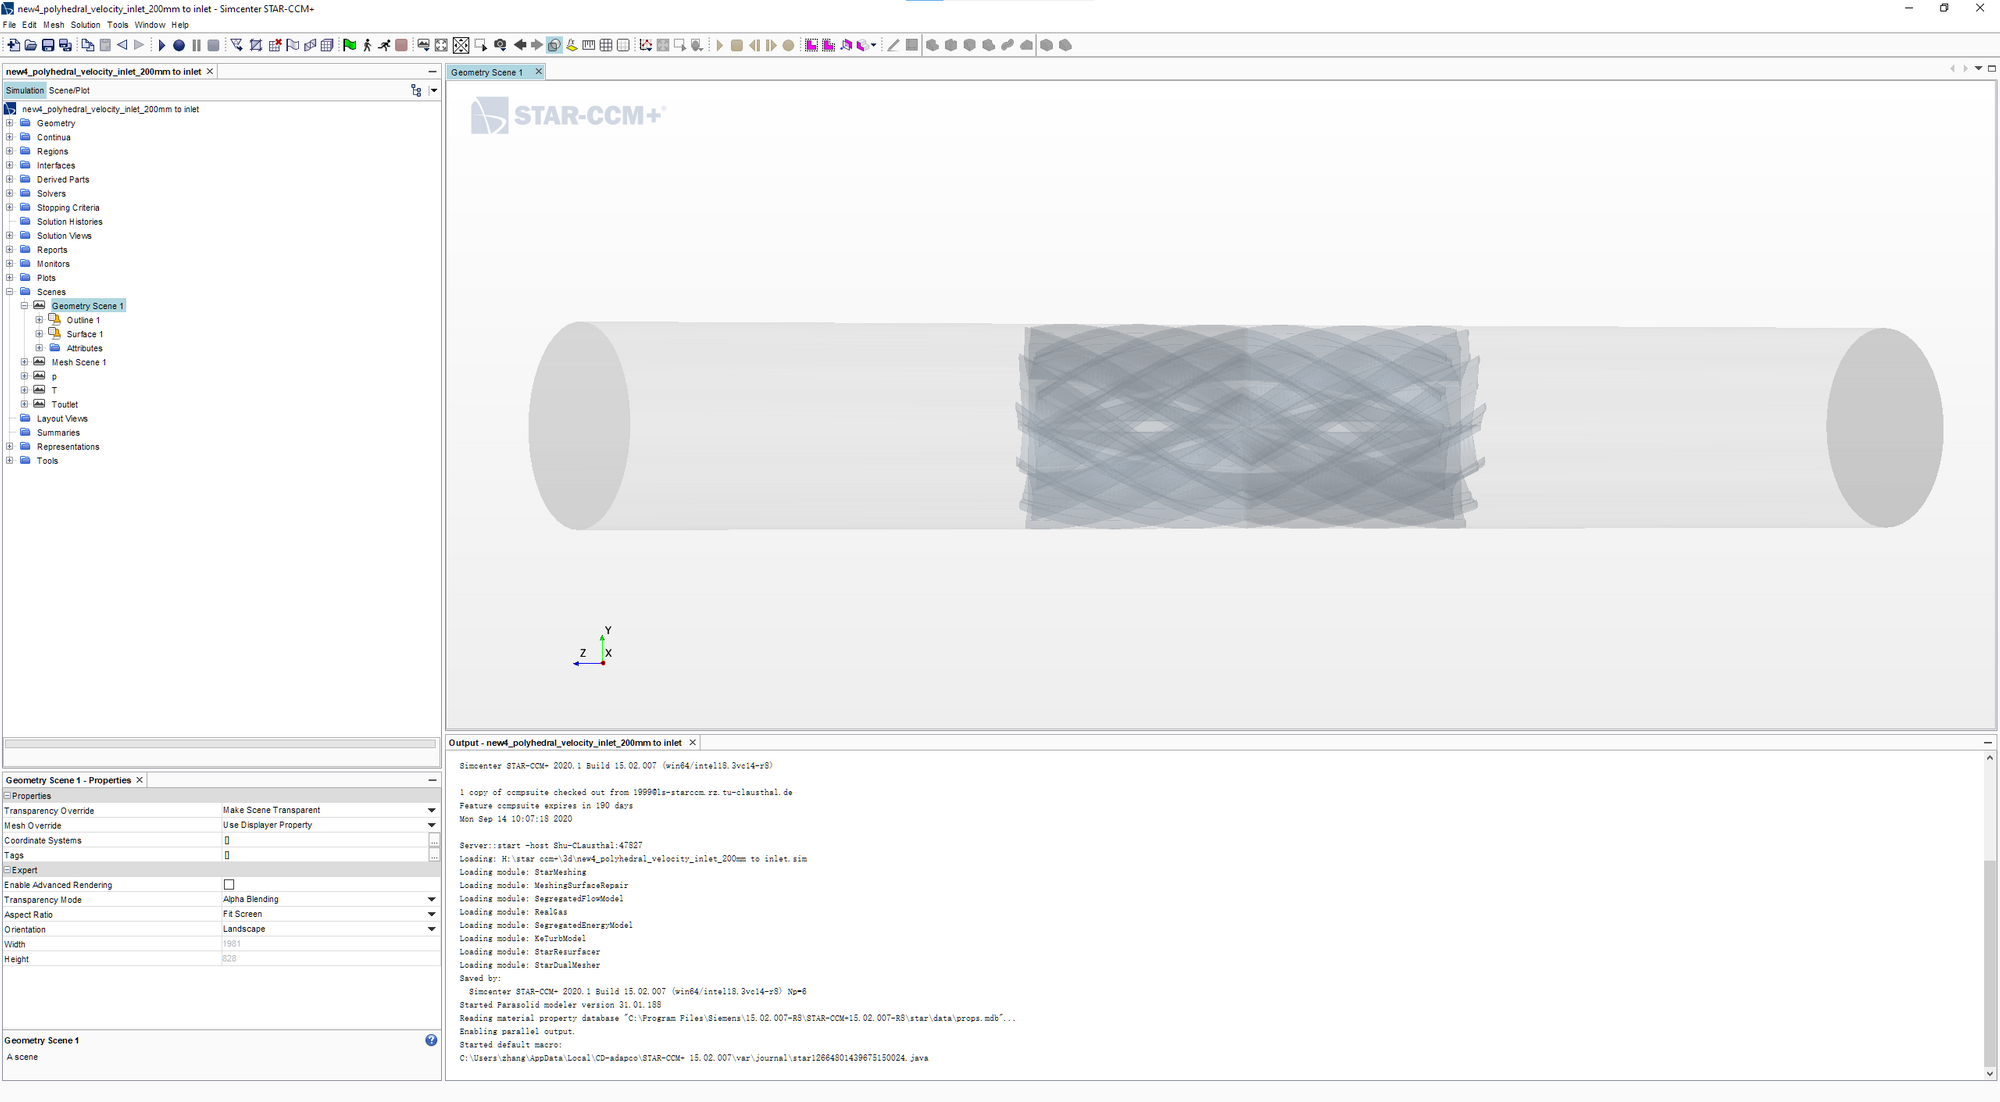
\includegraphics[width=\textwidth]{./docu_pictures/sketch.png}}
\end{center}
\caption{Below is a sketch of our simulation.}
\label{simulation-sketch}
\end{figure}

Static heat-exchanger is in the middle. 

Now we go further into details.


%%%%%%%%%%%%%%%%%%%%%%%%%%%%%%%%%%%%%%%%%%
\section{Conclusions}



%%%%%%%%%%%%%%%%%%%%%%%%%%%%%%%%%%%%%%%%%%
\vspace{6pt} 

%%%%%%%%%%%%%%%%%%%%%%%%%%%%%%%%%%%%%%%%%%
%% optional
%\supplementary{The following are available online at \linksupplementary{s1}, Figure S1: title, Table S1: title, Video S1: title.}

% Only for the journal Methods and Protocols:
% If you wish to submit a video article, please do so with any other supplementary material.
% \supplementary{The following are available at \linksupplementary{s1}, Figure S1: title, Table S1: title, Video S1: title. A supporting video article is available at doi: link.}

%%%%%%%%%%%%%%%%%%%%%%%%%%%%%%%%%%%%%%%%%%
\authorcontributions{}

%%%%%%%%%%%%%%%%%%%%%%%%%%%%%%%%%%%%%%%%%%
\funding{This research received no external funding}

%%%%%%%%%%%%%%%%%%%%%%%%%%%%%%%%%%%%%%%%%%
\acknowledgments{.}

%%%%%%%%%%%%%%%%%%%%%%%%%%%%%%%%%%%%%%%%%%
\conflictsofinterest{} 

%%%%%%%%%%%%%%%%%%%%%%%%%%%%%%%%%%%%%%%%%%
%% optional
\abbreviations{The following abbreviations are used in this manuscript:\\

\noindent 
\begin{tabular}{@{}ll}
MDPI & Multidisciplinary Digital Publishing Institute\\
DOAJ & Directory of open access journals\\
TLA & Three letter acronym\\
LD & linear dichroism
\end{tabular}}

%%%%%%%%%%%%%%%%%%%%%%%%%%%%%%%%%%%%%%%%%%
%% optional
\appendixtitles{yes} %Leave argument "no" if all appendix headings stay EMPTY (then no dot is printed after "Appendix A"). If the appendix sections contain a heading then change the argument to "yes".
\appendix
\section{Requirement Specification}
 \begin{table}[H]
\caption{Requirement specification list for the heat exchanger}
\centering
%% \tablesize{} %% You can specify the fontsize here, e.g., \tablesize{\footnotesize}. If commented out \small will be used.
\begin{tabular}{llllll}
\toprule
\textbf{\makecell{Obligatory\\or Desirable}} & \textbf{Category}	& \textbf{Description}	& \textbf{Value} & \textbf{\makecell{Person\\Responsible}} & \textbf{Last Changed} \\
\midrule
%    &   &   &  \\
Obligatory & Performance		& volume flow rate			& greater 0.5 m$^3$/h   & Scherf &  2020-06-23 \\
Obligatory    & Performance  & heat distribution  & radial and evenly   & Scherf & 2020-06-23 \\
Obligatory    & Performance  & heating water flowing trough  & from 10 °C to 80 °C   & Scherf & 2020-06-23 \\
Obligatory  & Performance   & low pressure drop &   & Scherf & 2020-06-23 \\
Obligatory	& Material    	& material temperature resistance			& between 0 °C and 90 °C   & Group A & 2020-06-23 \\
Obligatory	& Material    	& material water solvability  & unsolvable in water   & Group A & 2020-06-23 \\
Obligatory    & Material  & electrical conductivity  & greater $10^6$ S/m   & Group A & 2020-06-23 \\
Obligatory	& Manufacturing    	& manufacturing process  & additive manufacturing   & Scherf & 2020-06-23 \\
Desirable	& Geometry    	& customizability of model & model is parameterized   & Group A & 2020-06-23 \\
Obligatory	& Geometry    	& outer Shape  & cylindrical   & Group A & 2020-06-23 \\
Obligatory	& Geometry    	& outer diameter  &  94 mm   & Scherf & 2020-06-23 \\
Desirable	& Geometry    	& length  & up to 300 mm   & Scherf & 2020-06-23 \\
\sout{Obligatory}    & \sout{Geometry}  & \sout{outer wall}  & \sout{closed}   &   & 2020-06-23 \\
\sout{Desirable}    & \sout{Geometry}  & \sout{outer wall thickness} & \sout{smaller 5 mm}   &  & 2020-06-23 \\
Obligatory    & Geometry  & water flow direction  & fixed direction   & Scherf & 2020-06-23 \\


\bottomrule
\end{tabular}
\end{table}

\section{Simulation Model Requirement Specification}
 \begin{table}[H]
\caption{Requirement specification list for the heat exchanger simulation model}
\centering
%% \tablesize{} %% You can specify the fontsize here, e.g., \tablesize{\footnotesize}. If commented out \small will be used.
\begin{tabular}{llllll}
\toprule
\textbf{\makecell{Obligatory\\or Desirable}} & \textbf{Category}	& \textbf{Description}	& \textbf{Value} & \textbf{\makecell{Person\\Responsible}} & \textbf{Last Changed} \\
\midrule
%  &  &  &  &  &  \\
Desirable & Input		& file type & STL   & Group A &  2020-07-05 \\
Obligatory    & Input  &  fit within L=300 mm, D=94 mm cylinder &  & Group A &  2020-07-05 \\
Obligatory    & Input  &  material & ? & Group A &  2020-07-05 \\
%Obligatory    & Meshing  & ? & ? & Group A & 2020-07-05 \\
Obligatory & Simulation Geometry & tube & L=500 mm, D=94 mm cylinder & Group A & 2020-07-05 \\
Obligatory & Simulation Geometry & inlet Velocity & See Table A.1 & Group A & 2020-07-05 \\
Obligatory & Simulation Geometry & wall type & adiabatic & Group A & 2020-07-05 \\
Obligatory  & Output Values & pressure value at outlet & outlet pressure & Group A & 2020-07-05 \\
Obligatory & Output Pictures & \makecell{cut along the length and center of the\\cylinder showing velocity} & & Group A & 2020-07-05 \\
Obligatory & Output Pictures & \makecell{cut along the length and center of the\\cylinder showing temperature} & & Group A & 2020-07-05 \\
Obligatory & Output Pictures & at outlet showing temperature & & Group A & 2020-07-05 \\

\bottomrule
\end{tabular}
\end{table}

%%% Besprechung 09.06.2020 Notizen (+ markierte Punkte wurden in der Anforderungliste uebernommen):
% + Low pressure drop
% + Höhere Temperaturtoleranz, da das bauteil heißer wird als das Wasser#
% Effizienzgrad? Anderes Paper als Benchmark, oder verschiedene Versionen des eigenen Modells verbessern
% + Parametrisierbarkeit könnte Anforderung sein
% Statische Mischer als Anfangsstrukturen für Energieeintrag und Durchmischung
% + Länge des Zylinders: Festgelegt durch Versuchsaufbau und 3D-Drucker
% + Länge durch Versuchsaufbau: 1 m tube length - Ein- und Ablaufzone
% + Länge festgelegt: Bis 300 mm
% Druck dürfen wir selbst festlegen
% Befestigung im Rohr: Spaltmaß berücksichtigen, Fügemaße abschätzen, Befestigung durch Klemmringe (Eigentlich Sprengring innerhalb des Rohrs)
% + Es gibt feste Flußrichtung
% Anforderungen an das System stellen und auch an das Bauteil
% + Verantwortlichkeit fehlt in Anforderungsliste (3 Foliensatz)
% Aus welchem Material besteht das Rohr? Plexiglass PMMA, bis 90 °C Temperaturstabil
% Kleiners Rohr (1 Zoll) auch möglich für erste Versuche
% Anforderungsliste an Experimente.
% Leistung der Spule, Berchnen aus Anforderungen
% Anforderung, Wie radiale Wärme berechnen?

%%% Besprechung 16.06.2020
% Reduzierung der Durchflussmenge bei Liveversuch auf realistischere Werte
% Person responsible ist die Person für die die Anforderung erstellt wird
% Kupferspule ringsherum
% Performance Erhitzung des Wassers nur bis 80 °C
% Zylinder muss keine Hülle haben
% Bachelorarbeit Restriktionsgerechte Strukturoptimierung von additiv gefertigten Strukturreaktoren mit STar-ccm+, Lars Grobelny
% Datum der Änderungen mit in Anforderungsliste, da es benötigt wird
% Wir kriegen Fotos vom Versuchsstand
% Wir kriegen Simulationsmodell der Bachelorarbeit
% Anforderungsliste soll in den Anhang des Dokuments
% Zeitplanung bis spätestens nächste Woche vorlegen, mit Angabe, wer für was verantwortlich ist (gun chart?)
% Teile dürfen abbrechen von unserer Tube
% Funktionsmodell können wir schon anfangen mit z. B. Brainstorming was
% Funktionsmodell sollte in ca. 5 h zu machen sein
% Bis nächste Woche ein diskussionsfähiges Funktionsmodell vorlegen
% Projektplanung der nächsten Wochen vorstellen
% Nächste Besprechung Mittwoch 24.06.2020 um 10 Uhr 

%%% Besprechung 24.06.2020
% Optionen Wärmetest:
% 1. Wärmebildkamera, mit kalter Luft durchströmen und denn auf einen vertikalen Schnitt gucken
% 2. Thermoelemente einbauen, es gibt faserelektronisches Messsytem für Temperaturen
%    Miopas als Firma miopas.de
% Kleinerer Versuchsaufbau mit 1 Zoll Rohr möglich, selbe Sensoren (Druck) und ähnliches möglich
% Sobald die Ärzte die Kontaktdaten erhalten haben und kontakt hergestellt wurde kann es losgehen
% Sören am ehesten im IMW anrufen

%%% Besprechung 30.06.2020
% Statt Ansys können wir Star-CCM+ benutzen, da Sören sich deutlich besser damit auskennt
% Uns wurde nochmals angeboten irgendwas zu Drucken
% Plan für nächste Woche
% - Simulationsmodell für Wärmeeintrag fertigmachen
% - Anforderungsliste Simulationsmodell
% - Simulationsmodell für Druckverlust ?
% - Allererster Designentwurf als fertigungsgerechtes CAD-Modell

%%% Besprechung 07.07.2020
% Toleranz bei input geoemetrie dimensionen
% Mesch anhand minimaler geometrien 
% Netzstudie als Anforderung um zu validieren, dass das Mesch in Ordnung ist
% Fürs Cura mehr verbindung zu grundplatte
% Radiale Durchmischung verbessern
% Für nächste Woche
% Simulationsmodell verbessern, Mesch verbessern
% Was wollen wir experimentell machen, was in Model?
% Welche Teile unser Geometrie haben welchen Einfluss auf Ausgabeparameter

%%% Besprechung 13.07.2020
% Mesh-Dichte an Stegdichte anpassen
% Eher "ingenieurwerte" als Abbruchkriterium z. B. 

%%% Besprechung 21.07.2020
% Sandpapier um PLA abzutragen, vielleicht Drehbank
% Heatsource in Basissimulation deutlich sinnvoller als statische Temperatur
% Modell an Can schicken mit E-Mail der Probleme
% Strömungsgeschwindigkeit im Experiment später 
% Energieeintrag ins Bauteil wird später als E-Mail erklärt
% Fasersensoren noch nicht da
% Technische Daten der Faser kommen per E-Mail
% Strukturierung des Papers bis nächste Woche
% Leerrohrmessung kommt nächste Woche

%%% Besprechung 28.07.2020
% Leerrohrmessung Ergebnisse: Kommt noch...
% Induktionsspule Leistung: Es gibt zwei Stück, Sören guckt was die können, aber maximal 3500 Watt
% Lieber 3 Modelle gleichzeitig mit jeweils 2 Kernen rechnen
% Fasersensoren? 
% Pumpe ist Kreiselpumpe, hält Durchflussmenge ziemlich konstant
% Fertigungsrestriktionen für Metall-Drucker werden hochgeladen
% Sie haben einen neuen Drucker, der auch Keramik verarbeiten kann, ein Formlabs Form 2

%%% Besprechung 04.08.2020
% Faser hat 5 Messpunkte Abstand 20 mm oder 30 mm
% Düsen 0.25, 0.4, 0.6, 0.8 für Ultimaker verfügbar
% Netz umbauen auf Polyhedral
% Surfaces ignorieren

%%% Besprechung 11.08.2020
% Modell auf Fertigbarkeit überprüfen (z. B. Fertigungsrestriktionen tabellarisch abklappern)
% Hauptaussage AM-Bauteil bietet höheren Energieeintrag pro Volumen, ist schneller und einfacher zu fertigen
% Volumenstrom an Reynoldszahl festlegen
% Leerrohrmessung als Vergleichswert für Literaturvergleich
% Werte anderer statischer Mischer aus Literatur suchen zum Vergleich
% kenics Mischer vielleicht als Grundlage
% Freitag Leerrohr Validierung mit Literatur schicken, Energieeintrag mit Eisen durch Induktion (Effizienz, wie viel gebe ich drauf, wie viel kommt an), Leerrohrsimulation

%%%%%%%%%%%%%%%%%%%%%%%%%%%%%%%%%%%%%%%%%%
% Citations and References in Supplementary files are permitted provided that they also appear in the reference list here. 

%=====================================
% References, variant A: internal bibliography
%=====================================
\reftitle{References}
\begin{thebibliography}{999}
\bibitem{link-1}
https://zhuanlan.zhihu.com/p/89651311 (visited on 14.09.2020)
\bibitem{link-2}
https://uk.pcmag.com/3d-printers/74222/3d-printing-what-you-need-to-know (visited on 14.09.2020)
% Reference 1
\bibitem[Author1(year)]{ref-journal}
Author1, T. The title of the cited article. {\em Journal Abbreviation} {\bf 2008}, {\em 10}, 142--149.
% Reference 2
\bibitem[Author2(year)]{ref-book}
Author2, L. The title of the cited contribution. In {\em The Book Title}; Editor1, F., Editor2, A., Eds.; Publishing House: City, Country, 2007; pp. 32--58.
\end{thebibliography}

% The following MDPI journals use author-date citation: Arts, Econometrics, Economies, Genealogy, Humanities, IJFS, JRFM, Laws, Religions, Risks, Social Sciences. For those journals, please follow the formatting guidelines on http://www.mdpi.com/authors/references
% To cite two works by the same author: \citeauthor{ref-journal-1a} (\citeyear{ref-journal-1a}, \citeyear{ref-journal-1b}). This produces: Whittaker (1967, 1975)
% To cite two works by the same author with specific pages: \citeauthor{ref-journal-3a} (\citeyear{ref-journal-3a}, p. 328; \citeyear{ref-journal-3b}, p.475). This produces: Wong (1999, p. 328; 2000, p. 475)

%=====================================
% References, variant B: external bibliography
%=====================================
%\externalbibliography{yes}
%\bibliography{your_external_BibTeX_file}

%%%%%%%%%%%%%%%%%%%%%%%%%%%%%%%%%%%%%%%%%%
%% optional
%\sampleavailability{Samples of the compounds ...... are available from the authors.}

%% for journal Sci
%\reviewreports{\\
%Reviewer 1 comments and authors’ response\\
%Reviewer 2 comments and authors’ response\\
%Reviewer 3 comments and authors’ response
%}

%%%%%%%%%%%%%%%%%%%%%%%%%%%%%%%%%%%%%%%%%%
\end{document}

